\documentclass{tufte-handout}

\title{An Introduction to Git}

\author[Dr. Doeg]{The Invisible College}

%\date{28 March 2010} % without \date command, current date is supplied

%\geometry{showframe} % display margins for debugging page layout

\usepackage{graphicx} % allow embedded images
  \setkeys{Gin}{width=\linewidth,totalheight=\textheight,keepaspectratio}
  \graphicspath{{graphics/}} % set of paths to search for images
\usepackage{amsmath}  % extended mathematics
\usepackage{booktabs} % book-quality tables
\usepackage{units}    % non-stacked fractions and better unit spacing
\usepackage{multicol} % multiple column layout facilities
\usepackage{lipsum}   % filler text
\usepackage{fancyvrb} % extended verbatim environments
  \fvset{fontsize=\normalsize}% default font size for fancy-verbatim environments
  
  
  
    %MADNESS
  
  \usepackage[T1]{fontenc} % Use 8-bit encoding that has 256 glyphs
\usepackage{fourier} % Use the Adobe Utopia font for the document - comment this line to return to the LaTeX default
\usepackage[english]{babel} % English language/hyphenation
\usepackage{amsmath,amsfonts,amsthm} % Math packages
\usepackage{mathtools}% http://ctan.org/pkg/mathtools
\usepackage{etoolbox}% http://ctan.org/pkg/etoolbox
\usepackage{lipsum} % Used for inserting dummy 'Lorem ipsum' text into the template
\usepackage{units}% To use \nicefrac
\usepackage{cancel}% To use \cancel
\usepackage{physymb}%To use r
\usepackage{sectsty} % Allows customizing section commands
\usepackage[dvipsnames]{xcolor}
\usepackage{pgf,tikz}%To draw 
\usepackage{pgfplots}%To draw 
\usetikzlibrary{shapes,arrows}%To draw 
\usetikzlibrary{patterns,fadings}
 \usetikzlibrary{decorations.pathreplacing}%To draw curly braces 
 \usetikzlibrary{snakes}%To draw 
 \usetikzlibrary{spy}%To do zoom-in
 \usepackage{setspace}%Set margins and such
 \usepackage{3dplot}%To draw in 3D
\usepackage{framed}%To get shade behind text


\definecolor{shadecolor}{rgb}{0.9,0.9,0.9}%setting shade color
\allsectionsfont{\centering \normalfont\scshape} % Make all sections centered, the default font and small caps
  
  

  
  

% Standardize command font styles and environments
\newcommand{\doccmd}[1]{\texttt{\textbackslash#1}}% command name -- adds backslash automatically
\newcommand{\docopt}[1]{\ensuremath{\langle}\textrm{\textit{#1}}\ensuremath{\rangle}}% optional command argument
\newcommand{\docarg}[1]{\textrm{\textit{#1}}}% (required) command argument
\newcommand{\docenv}[1]{\textsf{#1}}% environment name
\newcommand{\docpkg}[1]{\texttt{#1}}% package name
\newcommand{\doccls}[1]{\texttt{#1}}% document class name
\newcommand{\docclsopt}[1]{\texttt{#1}}% document class option name
\newenvironment{docspec}{\begin{quote}\noindent}{\end{quote}}% command specification environment

\begin{document}

\maketitle% this prints the handout title, author, and date
\begin{marginfigure}%
  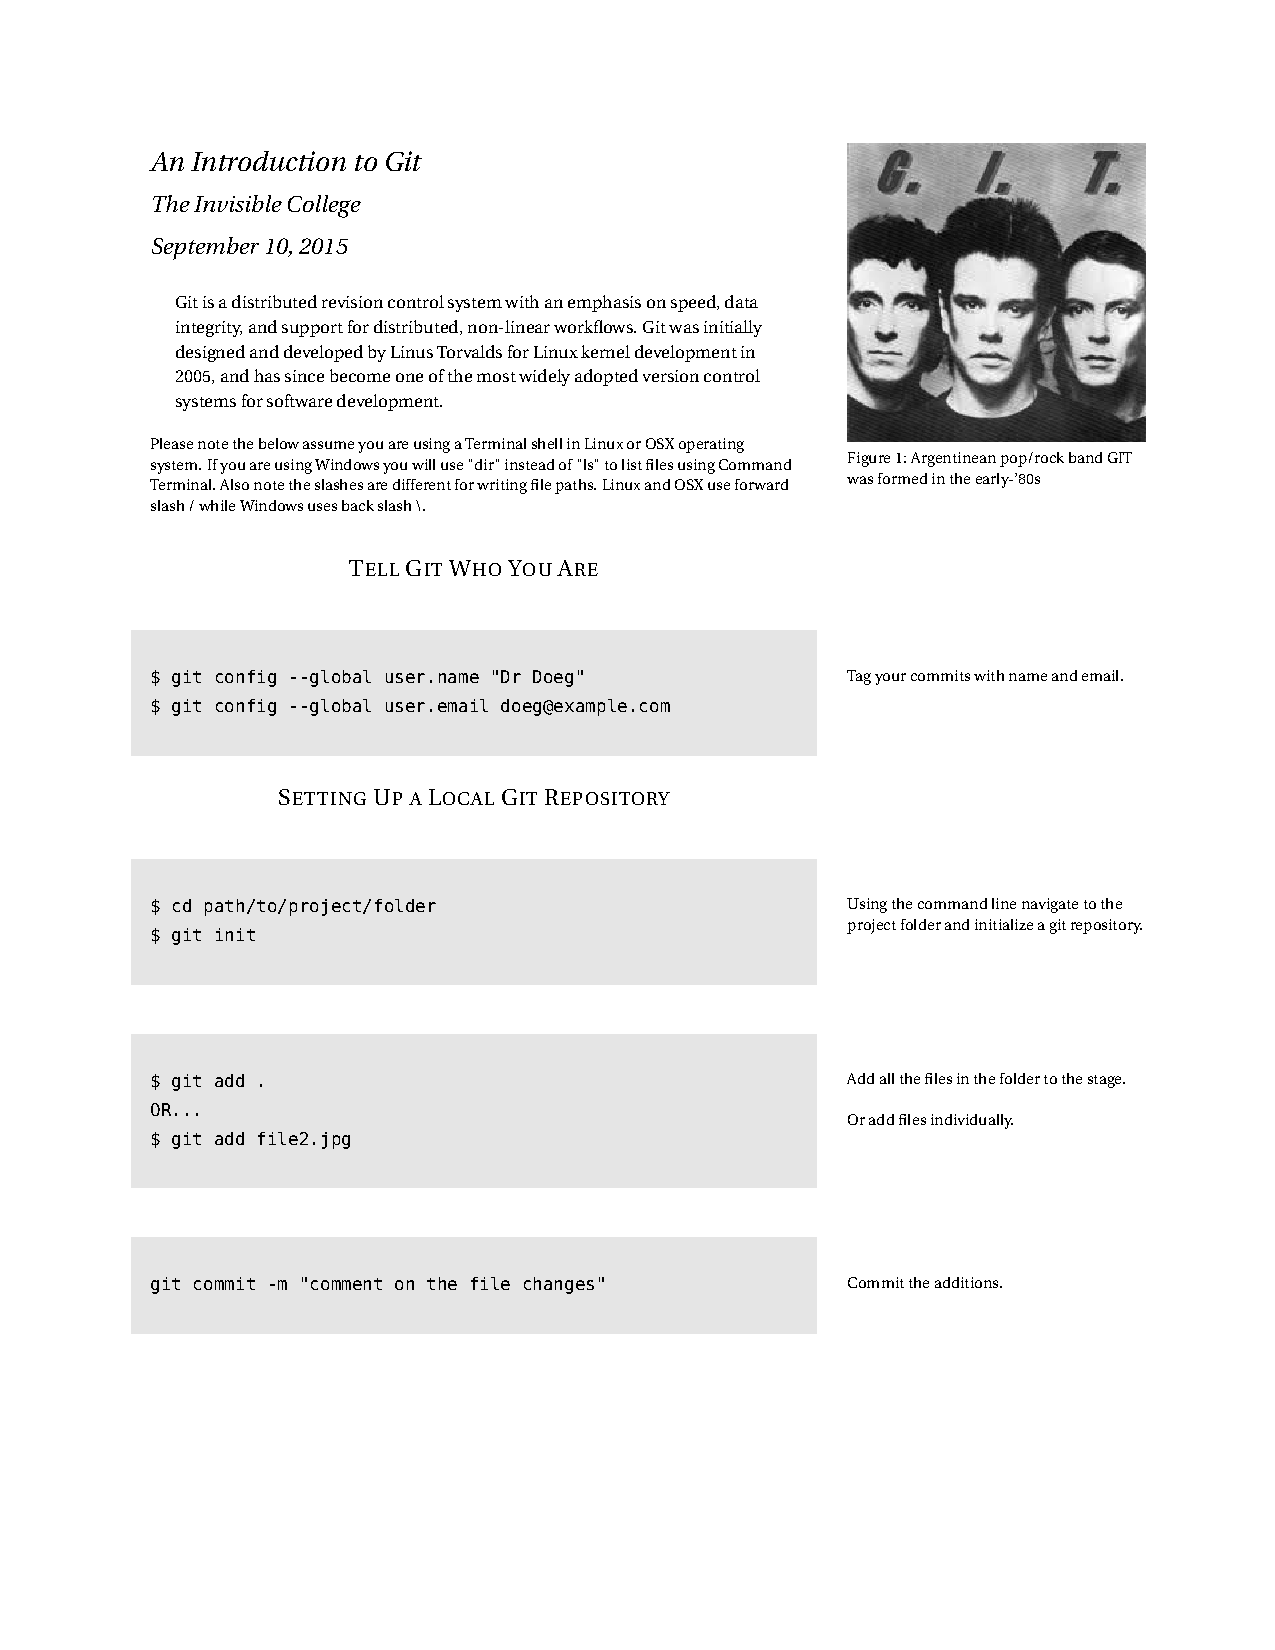
\includegraphics[width=\linewidth]{git.jpeg}
  \caption{Argentinean pop/rock band GIT was formed in the early-'80s}
  \label{fig:marginfig}
\end{marginfigure}
\begin{abstract}
\noindent
Git is a distributed revision control system with an emphasis on speed, data integrity, and support for distributed, non-linear workflows.  Git was initially designed and developed by Linus Torvalds for Linux kernel development in 2005, and has since become one of the most widely adopted version control systems for software development.
\end{abstract}

\noindent \footnotesize{Please note the below assume you are using a Terminal shell in Linux or OSX operating system.  If you are using Windows you will use "dir" instead of "ls" to list files using Command Terminal.  Also note the slashes are different for writing file paths.  Linux and OSX use forward slash / while Windows uses back slash \textbackslash.}

\normalsize
\section{Tell Git Who You Are}

\marginnote[40pt]{Tag your commits with name and email.}
\begin{shaded}
\begin{verbatim}
$ git config --global user.name "Dr Doeg"
$ git config --global user.email doeg@example.com
\end{verbatim}
\end{shaded}

\section{Setting Up a Local Git Repository}

\marginnote[40pt]{Using the command line navigate to the project folder and initialize a git repository.}

\begin{shaded}
\begin{verbatim}
$ cd path/to/project/folder
$ git init
\end{verbatim}
\end{shaded}

\marginnote[40pt]{Add all the files in the folder to the stage.\\ \ \\
\noindent Or add files individually.  }
\begin{shaded}
\begin{verbatim}
$ git add .
OR...
$ git add file2.jpg
\end{verbatim}
\end{shaded}

\marginnote[40pt]{Commit the additions.  }
\begin{shaded}
\begin{verbatim}
git commit -m "comment on the file changes"
\end{verbatim}
\end{shaded}



\newpage

\section{Push Your Local Repository to GitHub}

\marginnote[40pt]{\normalsize \bf{Setup the remote repository location on GitHub using your account.}}
\begin{shaded}
\begin{verbatim}
$ git remote add origin https://github.com/...
   YourAccount/WhatYouNamedTheRepo.git
$ git remote -v
\end{verbatim}
\end{shaded}

\marginnote[40pt]{Push the committed structure to the remote server.}
\begin{shaded}
\begin{verbatim}
$ git push origin master
\end{verbatim}
\end{shaded}




\section{Cloning an Existing Repository From GitHub }


\marginnote[40pt]{Navigate to the desired location in file structure.}
\begin{shaded}
\begin{verbatim}
$ cd path/to/whereUwant/folder
\end{verbatim}
\end{shaded}

\marginnote[40pt]{Set the location on the GitHub server to place the repositiory.}
\begin{shaded}
\begin{verbatim}
$ git clone https://github.com/YOUR-USERNAME/YOUR-REPOSITORY
\end{verbatim}
\end{shaded}

\section{Updating an Existing Repository From GitHub }

\marginnote[40pt]{Update the current project folder from the GitHub remote server.}
\begin{shaded}
\begin{verbatim}
$ git pull -u origin master
\end{verbatim}
\end{shaded}


\section{Get Git to Tell You Where It's At}

\marginnote[40pt]{Get information on the git repository.}
\begin{shaded}
\begin{verbatim}
$ git status
\end{verbatim}
\end{shaded}




\section{Get Git and Github}

\marginnote[20pt]{Download git and register an account at GitHub.}
https://git-scm.com/downloads  \\
\noindent https://github.com/ 

\section{More on Git}
\marginnote[20pt]{Look at the official documentation for more information.}
https://git-scm.com/book/en/v2

\bibliography{sample-handout}
\bibliographystyle{plainnat}



\end{document}
